\documentclass[12pt]{article}
\linespread{1.2}
\usepackage[margin=2cm]{geometry}
\usepackage[utf8]{inputenc}
\usepackage{amsfonts}
\usepackage{amsmath}
\usepackage{multicol}
\usepackage{amsthm}
\usepackage{amssymb,scrextend}
\usepackage{graphicx,tikz}
\newtheorem{dfn}{Definition}
\renewcommand{\qed}{\hfill$\blacksquare$}
\let\newproof\proof
\renewenvironment{proof}{\vspace{1em}\begin{addmargin}[2em]{0em}\begin{newproof}}{\end{newproof}\end{addmargin}\qed}
\newenvironment{theorem}[2][Theorem]{\begin{trivlist}
\item[\hskip \labelsep {\bfseries #1} \hskip \labelsep {\bfseries #2.}]}{\end{trivlist}}
\newenvironment{example}[2][Example]{\begin{trivlist}
\item[\hskip \labelsep {\bfseries #1} \hskip \labelsep {\bfseries #2.}]}{\end{trivlist}}
\newenvironment{lemma}[2][Lemma]{\begin{trivlist}
\item[\hskip \labelsep {\bfseries #1} \hskip \labelsep {\bfseries #2.}]}{\end{trivlist}}
\newenvironment{exercise}[2][Exercise]{\begin{trivlist}
\item[\hskip \labelsep {\bfseries #1} \hskip \labelsep {\bfseries #2}]}{\end{trivlist}}
\newenvironment{problem}[2][Problem]{\begin{trivlist}
\item[\hskip \labelsep {\bfseries #1} \hskip \labelsep {\bfseries #2.}]}{\end{trivlist}}
\newenvironment{corollary}[2][Corollary]{\begin{trivlist}
\item[\hskip \labelsep {\bfseries #1} \hskip \labelsep {\bfseries #2.}]}{\end{trivlist}}
\usepackage{fancyhdr,enumitem,changepage,url}

\pagestyle{fancy}
\author{Warren Atkison}
\date{\today}
\setlength{\headheight}{15pt}
\begin{document}
\fancyhf{}
\fancyhead[L]{Warren Atkison}
\fancyhead[C]{Homework Set 3}
\fancyhead[R]{\today}
\fancyfoot[R]{\thepage}

\begin{exercise}{1.6.6. (3pt)}
	Suppose five points are chosen from a square whose sides are length $s$. (The points may be either in the interior of the square or on the boundary.) Show that two of the points are at most $s\sqrt{2}/2$ apart. Find five points so that no two are less than $s\sqrt{2}/2$ apart. 
\end{exercise}
\begin{proof} Let the bottom left and corner of the square lie on (0,0).
	We can divide the square with side length $s$ into 4 sub-squares with side lengths $s/2$. By the pigeon hole principle, at least 2 points must lie inside a square of side length $s/2$. The distance between any two points $p = (x,y)$ can be given by
	\[
		d = \sqrt{(x_1 - x_2)^2 + (y_1 - y_2)^2}
	\]
	WLOG, let 2 points be located in the bottom left sub-square of side length $s/2$. To maximize $d$, we can set one point at $(s/2,s/2)$ and the other at $(0,0)$ which gives
	\[
		d = \sqrt{(s/2 - 0)^2 + (s/2 - 0)^2} = \sqrt{2(s/2)^2} = s\sqrt{2}/2
	\]
\end{proof} \\
One way to place all five points such that there distances are maximized is as follows 
\[
	A = (0,0),~B = (0,s),~C = (s/2,s/2),~D = (s,0),~E = (s,s)
\]
\begin{center}
	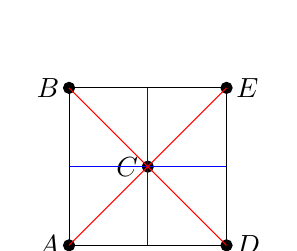
\begin{tikzpicture}

	\coordinate (A) at (0,0);
	\coordinate (B) at (0,2);
	\coordinate (C) at (1,1);
	\coordinate (D) at (2,0);
	\coordinate (E) at (2,2);

	%\foreach \vertex in {A,B,C,D,E}
		%\filldraw [black] (\vertex) circle (2pt);
	
	\filldraw [black] (A) circle (2pt) node[anchor=east] {$A$};
	\filldraw [black] (B) circle (2pt) node[anchor=east] {$B$};
	\filldraw [black] (C) circle (2pt) node[anchor=east] {$C$};
	\filldraw [black] (D) circle (2pt) node[anchor=west] {$D$};
	\filldraw [black] (E) circle (2pt) node[anchor=west] {$E$};




    % Draw horizontal lines
    \draw (0,0) -- (2,0);
    \draw[blue] (0,1) -- (2,1);
    \draw (0,2) -- (2,2);
    
    % Draw vertical lines
    \draw (0,0) -- (0,2);
    \draw[blue] (1,0) -- (1,2);
    \draw (2,0) -- (2,2);

    \draw[red] (A) -- (C);
    \draw[red] (C) -- (E);
    \draw[red] (C) -- (D);
    \draw[red] (B) -- (C);
	\end{tikzpicture}
\end{center}
\begin{exercise}{1.6.7. (3pt)}
	Show that if the edges of $K_6$ are colored with two colors, there are at least two monochromatic triangles. (Two triangles are different if each contains at least one vertex not in the other. For example, two red triangles that share an edge count as two triangles.) Color the edges of $K_6$ so that there are exactly two monochromatic triangles. 
\end{exercise}
\begin{proof}
	Since $R(3) = 6$, we know there must be at least one monochromatic triangle. Let these 3 vertices be $v_1$, $v_2$, and $v_3$, and the remaining three be $v_4$, $v_5$, and $v_6$. WLOG, let $v_1v_2v_3$ of color $C_1$ be the only monochromatic triangle. There must be an edge in $v_4v_5v_6$ of color $C_2$ otherwise we would have another monochromatic triangle, let this edge be $v_4v_5$. $v_4$ and $v_5$ must have 2 edges of color $C_2$ which connect to either $v_1$, $v_2$, or $v_3$ otherwise we would have 2 edges of color $C_1$ from $v_4$ or $v_5$ connecting to 2 points on the triangle $v_1v_2v_3$ which would form another monochromatic triangle. However, then $v_4$ and $v_5$ have 2 edges of color $C_2$ each which connect to either $v_1$, $v_2$, or $v_3$, so there are 4 edges of color $C_2$ and 3 points and by the pigeonhole principle 2 edges of color $C_2$ from $v_4$ and $v_5$ must connect to the same point in $v_1v_2v_3$ which forms a monochromatic triangle and we have a contradiction. 
\begin{center}
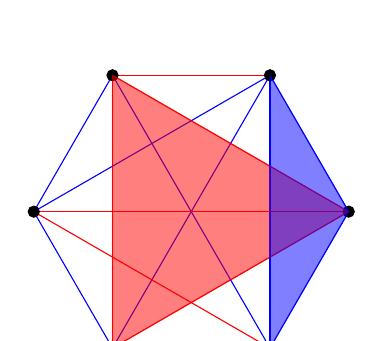
\begin{tikzpicture}
    % Define vertices of the hexagon
    \coordinate (A) at (0,0);
    \coordinate (B) at (2,0);
    \coordinate (C) at (3,1.732);
    \coordinate (D) at (2,3.464);
    \coordinate (E) at (0,3.464);
    \coordinate (F) at (-1,1.732);
    
    % Draw the hexagon
    \draw[red] (A) -- (B);
    \draw[blue] (B) -- (C);
    \draw[blue] (C) -- (D);
    \draw[red] (D) -- (E);
    \draw[blue] (E) -- (F);
    \draw[blue] (F) -- (A);
    
    % Draw edges connecting vertices with different colors
    \draw[red] (A) -- (C);
    \draw[red] (C) -- (E);
    \draw[red] (E) -- (A);
    \draw[blue] (B) -- (D);
    \draw[blue] (A) -- (D);
    \draw[blue] (B) -- (E);
    \draw[red] (F) -- (C);
    \draw[red] (B) -- (F);
    \draw[blue] (F) -- (D);

    
    % Mark vertices
    \foreach \vertex in {A, B, C, D, E, F}
        \filldraw [black] (\vertex) circle (2pt);
    
    % Inscribed triangles
    \filldraw[red, opacity=0.5] (A) -- (C) -- (E) -- cycle;
    \filldraw[blue, opacity=0.5] (B) -- (C) -- (D) -- cycle;
\end{tikzpicture}	
\end{center}
\end{proof}
\begin{exercise}{1.4.2. (2pt)}
	 Suppose $n$ is a square-free number, that is, no number $m^2$ divides $n$; put another way, square-free numbers are products of distinct prime factors, that is, $n=p_1p_2\ldots p_k$, where each $p_i$ is prime and no two prime factors are equal. Find the number of factorizations of $n$. For example, $30=2\cdot3\cdot5$, and the factorizations of 30 are 30, $6\cdot5$, $10\cdot3$, $2\cdot15$, and $2\cdot3\cdot5$. Note we count 30 alone as a factorization, though in some sense a trivial factorization. 
\end{exercise}	
We are essentially partitioning the factors on $n$, as we always use all the prime factors, we are just grouping them differently. Therefore, the number of factors for a square free number $n = p_1p_2 \ldots p_k$ is going to be equal to the number of ways to partition a $k$ set of elements, or $B_k$
\begin{exercise}{1.6.3. (2pt)}
	Each of 15 red balls and 15 green balls is marked with an integer between 1 and 100 inclusive; no integer appears on more than one ball. The value of a pair of balls is the sum of the numbers on the balls. Show there are at least two pairs, consisting of one red and one green ball, with the same value. Show that this is not necessarily true if there are 13 balls of each color. 
\end{exercise}
\begin{proof}
	Because each number is distinct, we have a total of $15 \cdot 15 = 225$ sums with one red and one green ball, and since the balls range from 1-100, the minimum sum is 3 and the maximum sum is 199 for a total of 197 possible sums. By the pigeonhole principle, there must be at one sum that occurs twice. For 13 balls, there are only $13 \cdot 13 = 169$ possible combinations, so the pigeonhole principle does not apply. 
\end{proof}
\begin{exercise} {1.6.1. (1pt)}
	Assume that the relation "friend'' is symmetric. Show that if $n \ge 2$, then in any group of n people there are two with the same number of friends in the group. 
\end{exercise}
\begin{proof}
	Since a person cannot be friends with themself, the maximum number of friends a person can have is $n - 1$ and the minimum is 0. However, if a person has $n - 1$ friends, then no one can have 0 friends and vis versa for a total of $n - 1$ possible number of friends any person can have. Thus, by the pigeonhole principle, at least 2 people have the same number of friends.
\end{proof}
\begin{exercise}{1.4.4. (1pt)}
	Find a recurrence relation for $S(n,k)$ (Sterling numbers of the second kind). Your recurrence should allow a fairly simple triangle construction containing the values $S(n,k)$, and then the Bell numbers may be computed by summing the rows of this triangle. Show the first five rows of the triangle, $n\in \{1,2,\ldots,5\}$. 	
\end{exercise}
\begin{align*}
	S(n+1,k) = S(n,k-1) + kS(n,k)
\end{align*}
If we are putting our new $n+1$ element into its own part, then there are $S(n,k-1)$ ways to arrange the other elements. If we put the $n+1$ element into an existing part, then we have $S(n,k)$ ways to arrange the rest of the elements for each part, so $kS(n,k)$ ways total. 
\[
\begin{array}{cccccc}
	1 &  &  &  &  &  \\
	 & 1 &  &  &  &  \\
	 & 1 & 1 &  &  &  \\
	 & 1 & 3 & 1 &  &  \\
	 & 1 & 7 & 6 & 1 &  \\
	 & 1 & 15 & 25 & 10 & 1
\end{array}
\]
\end{document}
